\chapter{Modelagem matemática}

\section{Modelagem matemática}

Dentro da pesquisa, foram realizadas duas modelagens distintas, ambas, diferentemente da literatura clássica, foram elaboradas com base nas estações de origem e destino, e não nos legs do percurso.

Para compreender essas propostas, consideremos uma versão simplificada do problema como se mostra na figura \ref{fig: fig1}, onde temos:

\begin{itemize}
	\item 4 estações pelas quais o trem deve passar em um único sentido, ou seja, o trem não tem retorno.
	\item O trem tem uma capacidade máxima de assentos.
	\item Há apenas um tipo de classe comercial.
	\item Existe apenas um período no horizonte de reserva.
	\item A variável de decisão é a quantidade de assentos que pode ser disponibilizada para venda em um trecho com origem e destino específicos.
	\item Todos os assentos disponibilizados para venda serão vendidos.
\end{itemize}

\begin{figure}[th]
	\begin{center}
		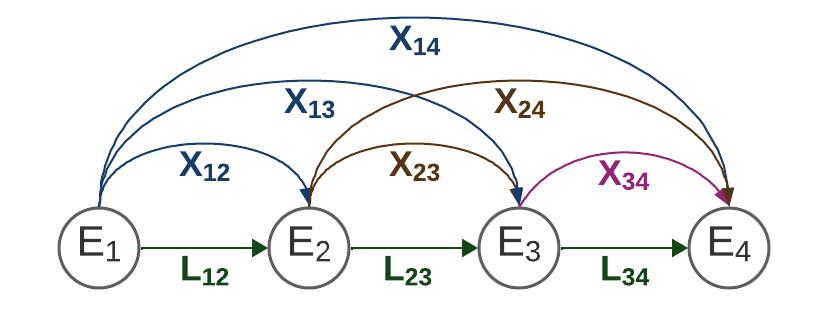
\includegraphics[scale=0.7]{img/fig1.png}
		\caption{Versão gráfica simples}
		% Fonte:~\cite{khaksar2013genetic}}
		\label{fig: fig1}
	\end{center}
\end{figure}


\section{Primeira modelagem matemática}\label{sec:modelo1}

Agora, para a primeira proposta de modelagem, temos o seguinte

\noindent $x_{ij}$: Quantidade de assentos que serão seguradas no trecho com origem em $i$ e destino em $j$, onde $j>i$ \\
\noindent $A_i$: Disponibilidade do trem na estação $i$ \\
\noindent $P_{ij}$: Preço da passagem no trajeto com origem em $i$ e destino em $j$ \\
\noindent $Q$: Capacidade do trem

Dado o exposto, a função objetivo será maximizar o lucro para cada possível venda em cada trajeto $i,j$, matematicamente seria:

$FO: max \quad x_{12}P_{12} + x_{13}P_{13} + x_{14}P_{14} + x_{23}P_{23} + x_{24}P_{24} + x_{34}P_{34}$

s.a.

Estação 1: $x_{12} + x_{13} + x_{14} \leq A_1 \quad onde \quad A_1 = Q $ \\
\indent Estação 2: $x_{23} + x_{24}  \leq  A_2 \quad onde \quad A_2 = A_1 - (x_{12} + x_{13} + x_{14}) + x_{12} $ \\
\indent Estação 3: $x_{34} \leq A_3 \quad onde \quad A_3 = A_2 - (x_{23} + x_{24}) + x_{13} + x_{23} $

Note que as restrições são aplicadas para cada uma das três primeiras estações, E1, E2 e E3, já que são as estações que têm pelo menos um destino, e a última estação, E4, é excluída, pois não possui nenhum destino.

Cada uma das restrições leva em consideração o fluxo de pessoas que sairão e entrarão no trem. Levando isso em conta, é necessário calcular a disponibilidade do trem para cada estação. Considere uma solução viável para o modelo, conforme mostrado na figura \ref{fig: fig2}, com uma capacidade total de 100 assentos para um trem.

\begin{figure}[!ht]
	\begin{center}
		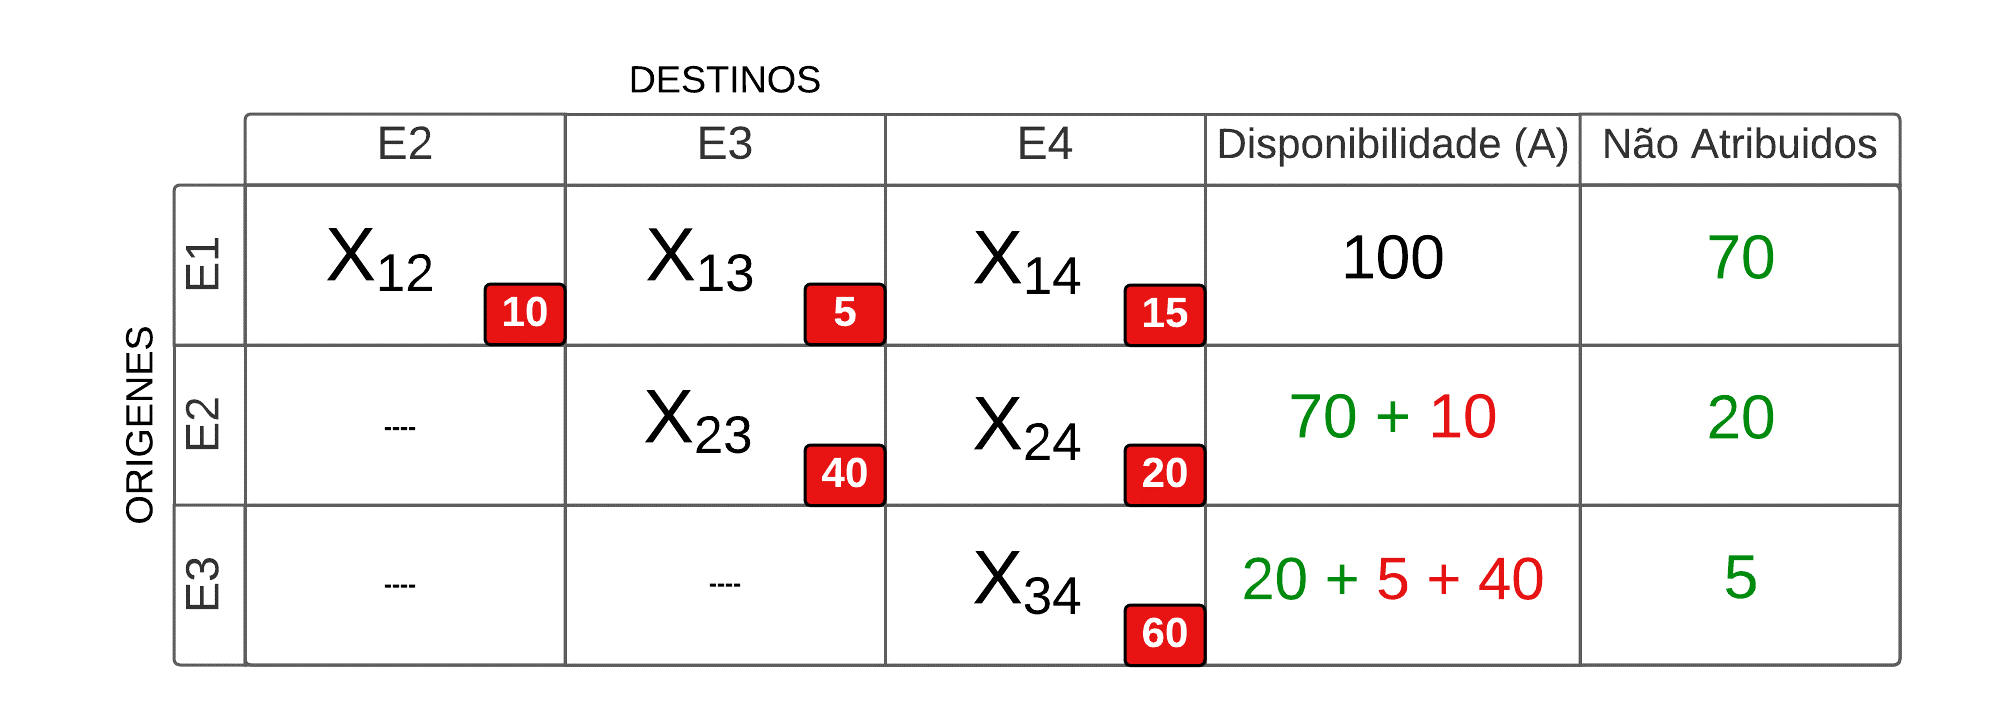
\includegraphics[scale=0.4]{img/fig2.png}
		\caption{Solução factível para o problema simplificado}
		% Fonte:~\cite{khaksar2013genetic}}
		\label{fig: fig2}
	\end{center}
\end{figure}

Note que, para a restrição da estação 1, o trem está com todos os assentos vazios, ou seja, \(A_1=100\), e que a soma das variáveis seria \(x_{12} + x_{13} + x_{14} = 10 + 5 + 15 = 30\). Portanto, teríamos \(30 \leq 100\), ou seja, foram disponibilizados para venda 30 assentos dos 100 que o trem possui. Nesse sentido, no momento da partida do trem da estação 1, haveria 70 assentos vazios ou disponíveis para venda em estações posteriores.

Agora, para a estação 2, teríamos \(A_2 = 100 - 30 + 10 = 70 + 10 = 80\). Já era conhecido que havia 70 assentos disponíveis vindos da estação 1, mas também é preciso levar em conta que os assentos com destino à estação 2 também ficarão disponíveis da estação 2 em diante, para este caso \(x_{12} = 10\). Portanto, para a estação 2, teríamos 80 assentos vazios para disponibilizar, ou seja, \(60 \leq 80\). Analogamente, o mesmo raciocínio seria aplicado para a estação 3, ou seja, teríamos a soma de todos os assentos que chegaram à estação 3, \(x_{13} = 5\) e \(x_{23} = 40\), assim teríamos \(A_3 = 80 - 60 + 5 + 40 = 20 + 5 + 40 = 65\), e no final teríamos \(60 \leq 65\).

Dada a lógica anterior, vejamos agora o modelo proposto completo:

\begin{table}[h]
	\centering
	\small
	\begin{tabular}{p{2cm} p{9.5cm} p{3.2cm}}
		\toprule
		\textbf{Definição} & \textbf{Notação}                                                                                                                                            & \textbf{Domínio}                             \\ \midrule
		\multicolumn{3}{l}{\textbf{Conjuntos}}                                                                                                                                                                                          \\ \midrule
		$OD$               & Conjunto de Trechos com itinerario                                                                                                                          &                                              \\
		$NAD$              & Conjunto de Trechos que NÃO são Adjacentes e que tem itinerario                                                                                             &                                              \\
		$BRI_{(o,d)}$      & Conjunto de Trechos contidos dentro de cada trecho $(o,d)$ NÃO Adjacente                                                                                    &                                              \\
		$V$                & Conjunto de Cabines do trem                                                                                                                                 &                                              \\
		$K_v$              & Conjunto de Classes de Control de cada cabine em $V$                                                                                                        &                                              \\
		$T$                & Conjunto de Check-Points (Períodos)                                                                                                                         &                                              \\ \midrule
		\multicolumn{3}{l}{\textbf{Parâmetros}}                                                                                                                                                                                         \\ \midrule
		% $n$                & Quantidade de Estações                                                                                                                                                 &                                              \\
		$Q$                & Capacidade do trem                                                                                                                                          &                                              \\
		$P_{ijvk}$         & Preços  das passagem no Trecho $(i,j)$, Cabine $v$ e Classe de Control $k$                                                                                  & $(i,j) \in OD,v \in V, k \in K_v$            \\
		$D_{ijvkt}$        & Demanda  das passagem no Trecho $(i,j)$, Cabine $v$ e Classe de Control $k$                                                                                 & $(i,j) \in OD,v \in V, k \in K_v, t \in T$   \\ \midrule
		\multicolumn{3}{l}{\textbf{Variáveis de decisão}}                                                                                                                                                                               \\ \midrule
		$A_{i}$            & Disponibilidade de passagens para vendas na estação i                                                                                                       & $i \in I$                                    \\
		$X_{ijvkt}$        & Quantidade de passagem atribuídos no trecho $(i,j)$, cabine $v$ e com classe de control $k$ no período $t$                                                  & $(i,j) \in OD, v \in V, k \in K_v, t \in T$  \\
		$Y_{ijvkt}$        & Quantidade de passagem autorizados no trecho $(i,j)$, cabine $v$ e com classe de control $k$ no período $t$                                                 & $(i,j) \in OD, v \in V, k \in K_v, t \in T$  \\
		% $BAL_{ijvt}$       & É uma variavel binaria que toma o valor de 1 quando $\sum_{k \in K_v }Y_{ijvkt} \neq 0$ e toma  valor de 0 caso contrario                                              & $(i,j) \in OD, v \in V, t \in T$             \\
		$BNA_{ijvkt}$      & É uma variavel binaria que toma o valor de 1 quando $Y_{ijvkt} \neq 0$ e toma  valor de 0 caso contrario, aplica-se apenas a trechos que não são adjacentes & $(i,j) \in NAD, v \in V, k \in K_v, t \in T$ \\
		% $Z_{ijvkt}$        & É uma variável real que assumirá três valores \{-1,0,1\}, é 1 quando a classe k da variável $Y_{ijvkt}$ é a última a assumir um valor, caso contrário pode ser -1 ou 0 & $(i,j) \in NAD, v \in V, k \in K_v, t \in T$ \\
		\bottomrule
	\end{tabular}
	\caption{Notação matemática}
	\label{tab: m1_definicao}
\end{table}


\begin{align}
	 & Max \quad Z = \sum_{(i,j)\in OD} \sum_{v\in V} \sum_{k\in K_v} \sum_{t\in T} P_{ijvk} X_{ijvkt}                                                                                                                \label{eq: m1_fo}                          \\
	 & \text{s.a.}  \notag                                                                                                                                                                                                                                       \\
	 & A_{i} = A_{i-1} - \sum_{(i,j) \in OD/j \geq i} \sum_{v\in V} \sum_{k\in K_v}\sum_{t\in T}X_{i-1,j,v,k,t} + \sum_{(i,j) \in OD/j<i}\sum_{v\in V} \sum_{k\in K_v}\sum_{t\in T}X_{jivkt}, \quad \forall i \in OD  \label{eq: m1_disponi}                     \\
	 & \sum_{(i,j) \in OD}\sum_{v\in V} \sum_{k\in K_v}\sum_{t\in T} X_{ijvkt} \leq A_{i} , \quad \forall i \in OD /i<j, i < n                                                                                        \label{eq: m1_cap_assig}                   \\
	 & Y_{ijvkt} \geq Y_{i,j,v,k+1,t},  \quad \forall (i,j),v,k,t / i < j, k < \lVert K_v \rVert,  P_{ijvk} \geq P_{i,j,v,k+1}                                                                                        \label{eq: m1_jerar_class}                 \\
	 & X_{ijvkt} \leq D_{ijvkt},  \quad \forall (i,j),v,k,t/ i < j                                                                                                                                                    \label{eq: m1_assig_menor_dem}             \\
	 & \sum_{(i,j) \in OD}\sum_{v\in V}\sum_{t\in T} Y_{i,j,v,k,t} \leq Q, \quad  k = min\{K_v\}, \forall i \in OD                                                                                                    \label{eq: m1_cap_autho_1er_class}         \\
	 & Y_{i,j,v,k,t} \geq  X_{i,j,v,k,t},  \quad k = max\{K_v\}, \forall(i,j),v,t                                                                                                                                     \label{eq: m1_autho_mayor_assig_1er_class} \\
	 & Y_{i,j,v,k,t} \geq  X_{i,j,v,k,t} + Y_{i,j,v,k + 1,t} , \forall(i,j),v, k, t / k < \lVert K_v\rVert                                                                                                            \label{eq: m1_autho_mayor_assig_mas_autho} \\
	%  & \text{Restrições de xxxx}  \notag                                                                                                                                                                                                                       \\
	%  & BAL_{i,j,v,t} \leq \sum_{k \in K_v}Y_{i,j,v,k,t} \leq BAL_{i,j,v,t} Q, \quad  \forall (i,j)\in OD,v,t                                                                                                        \label{eq: m1_activ_bin_sum_autho}         \\
	 & BNA_{o,d,v,k,t} \leq Y_{o,d,v,k,t} \leq BNA_{o,d,v,k,t} Q, \quad  \forall (o,d)\in NAD, v, k, t                                                                                                                \label{eq: m1_activ_bin_autho}             \\
	 & BNA_{o,d,v,k,t} \leq Y_{i,j,v,k,t} \leq BNA_{o,d,v,k,t} Q, \quad  \forall (o,d)\in NAD, (i,j) \in BRI_{(o,d)}, v,k,t                                                                                           \label{eq: m1_autho_igualar_trecho_maior}  \\
	%  & BNA_{o,d,v,k,t} + BNA_{o,d,v,k-1,t} -  BNA_{o,d,v,k+1,t} -1 = Z_{o,d,v,k,t}, \quad  \forall (o,d)\in NAD, v, t, k / \lVert K_v \rVert \geq 3                                                                 \label{eq: m1_cal_betwen_autho_val}        \\
	%  & BNA_{o,d,v,k,t} -  BNA_{o,d,v,k+1,t} = Z_{o,d,v,k,t}, \quad  \forall (o,d)\in NAD, v, t, k = min\{K_v\}                                                                                                      \label{eq: m1_cal_first_autho_val}         \\
	%  & BNA_{o,d,v,k,t} = Z_{o,d,v,k,t}, \quad  \forall (o,d)\in NAD, v, t, k = max\{K_v\}                                                                                                                           \label{eq: m1_cal_last_autho_val}          \\
	%  & Y_{i,j,v,k,t} \geq Z_{o,d,v,k,t} - (1-BAL_{i,j,v,t}), \quad  \forall (o,d)\in NAD, (i,j) \in BRI_{(o,d)}, v,t,k                                                                                              \label{eq: m1_autho_activ_noadj}           \\%[15pt]
	%  & \text{Restrições de inicialização}  \notag                                                                                                                                                                                                              \\
	 & X_{0,j,v,k,t} = 0,     \quad \forall j,k,t                                                                                                                                                                     \label{eq: m1_ini_assig}                   \\
	 & A_{0} = Q                                                                                                                                                                                                      \label{eq: m1_ini_disponi}                 \\
	%  & \text{Restrições de dominio}  \notag                                                                                                                                                                                                                   \\
	 & X_{ijvkt} \in \mathbb{Z}^+                                                                                                                                                                                     \label{eq: m1_dom_assig}                   \\
	 & Y_{ijvkt} \in \mathbb{Z}^+                                                                                                                                                                                     \label{eq: m1_dom_autho}                   \\
	 & A_{j} \in \mathbb{Z}^+                                                                                                                                                                                         \label{eq: m1_dom_disponi}                 \\
	%  & BAL_{ijvt} \in \{0,1\}                                                                                                                                                                                       \label{eq: m1_dom_bin_all}                 \\
	 & BNA_{ijvkt} \in \{0,1\}                                                                                                                                                                                        \label{eq: m1_dom_bin_nadja}
	%  & Z_{ijvkt} : Livre                                                                                                                                                                                            \label{eq: m1_dom_bin_true_last_value}
\end{align}


Na equação \ref{eq: m1_fo}, a qual representa a função objetivo, temos a soma do produto entre a quantidade de assentos atribuídos a cada trajeto de origem e destino para a classe comercial em cada período e cada vagone, multiplicada pelo preço correspondente para cada trajeto e classe, observe que queremos maximizar os ingressos em função dos asientos que estão atribuídos, que é o mais próximo que se tem da realidade em função da demanda conhecida.

A restrição \ref{eq: m1_disponi} é utilizada para calcular a disponibilidade de assentos de cada estação de origem, em cada período de tempo para cada classe em cada vagone e é a generalização do exemplo simplificado para calcular a variável de decisão $A_i$.

A restrição \ref{eq: m1_cap_assig} garante que todas as autorizações habilitadas a partir de cada estação de origem para cada período e cada classe de cada vagão não excedam a disponibilidade da sua estação de origem correspondente (a disponibilidades é calculada na restrição \ref{eq: m1_disponi}).

A restrição \ref{eq: m1_jerar_class} é uma restrição de hierarquia e garante que as quantidades de autorizações para as classes de maior preço sejam sempre maiores do que as quantidades de autorizações de menor preço em cada vagone, em cada trecho, e em  cada período do horizonte de reserva.

A restrição \ref{eq: m1_assig_menor_dem} garante que a quantidade de atribuições não ultrapasse a demanda para cada trecho de cada classe em cada vagoen e em cada período no horizonte de reserva.

A restrição \ref{eq: m1_cap_autho_1er_class} garanta que a soma de autorizações da classe mais costosa de cada vagone, de cada estação de origem, de tudos os periodos, não ultrapase a capacidade do trem, note que apenas estamos considerando a classe mais cara devido à natureza cumulativa das variáveis de autorização é por isso que o valor de k é o mínimo das classes de cada vagão, pois a ordem do nome das classes é crescente mas o seu valor é decrescente. Para melhor compreensão, suponhamos uma solução para um problema de dois vagones V1 e V2, 8 classes para V1 e 6 classes para V2, 10 trechos, um período e uma capacidade para 100 cadeiras, conforme mostra a figura \ref{fig: autorization}.

\begin{figure}[!ht]
	\begin{center}
		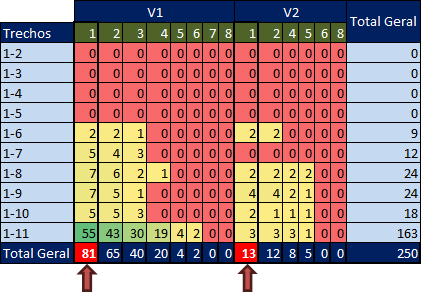
\includegraphics[scale=0.7]{img/autorization.png}
		\caption{Solução factível para a variavel de desição Autorização}
		% Fonte:~\cite{khaksar2013genetic}}
		\label{fig: autorization}
	\end{center}
\end{figure}

Observe que os nomes das classes são números ordenados em ordem crescente [1, 2, 3, ...] também o valor da classe 1 é mais caro que o valor da classe 2 e este é maior que o valor da classe 3 e assim por diante. Alem disso, a soma que não ultrapassará a capacidade do trem é a soma das classes 1 de cada vagone ou seja 81 + 13 que é menor a 100. Enquanto a soma total geral não teria sentido, uma vez que cada classe mais à direita conterá todas as classes à esquerda.


Até ao momento foi referido que a variável $Y$ tem um carácter cumulativo e são as restrições \ref{eq: m1_autho_mayor_assig_1er_class} e \ref{eq: m1_autho_mayor_assig_mas_autho} que controlam este comportamento. A restrição \ref{eq: m1_autho_mayor_assig_1er_class} é um caso particular da restrição \ref{eq: m1_autho_mayor_assig_mas_autho}, aplicada apenas à última classe, ou classe mais barata, segurada para cada vagão, ($k=max\{K_v\}$) e garante que a soma de todos os períodos, de cada trecho da classe mais barata da variável "autorização " é maior ou igual à variável de decisão "segurada" nas mesmas condições. Por outro lado, a restrição \ref{eq: m1_autho_mayor_assig_1er_class} garante que cada classe autorizada mais à esquerda seja sempre maior ou igual à classe autorizada imediatamente à sua direita mais a quantidade segurada da mesma classe, isto pela soma de todos os períodos, cada trecho e cada classe. Para melhor compreensão, assuma as mesmas suposições que foram feitas na restrição \ref{eq: m1_cap_autho_1er_class} %com a diferença que agora as tabelas representam uma solução factivel para a soma de n períodos e não um único período.


\begin{figure}[h!]
	\centering
	\begin{subfigure}[b]{0.450\linewidth}
		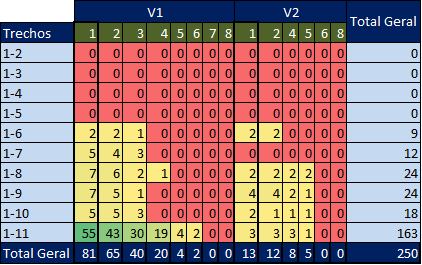
\includegraphics[width=\linewidth]{img/auto_sf.png}
		\caption{Autorização [Variavel $Y$]}
		\label{fig:auto_assig_a}
	\end{subfigure}\hspace{5mm}
	\begin{subfigure}[b]{0.434\linewidth}
		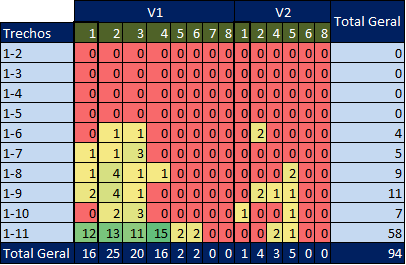
\includegraphics[width=\linewidth]{img/assig_sf.png}
		\caption{Atribução [Variavel $X$]}
		\label{fig:auto_assig_b}
	\end{subfigure}
	\caption{Solução factível para as variaveis de desição Autorização e Atribução}
	\label{fig:auto_assig}
\end{figure}

Observe a linha correspondente ao trecho 1-11 do vagão V2 na tabela \ref{fig:auto_assig_b}, veja que a classe segurada mais barata foi a classe 5 com valor 1, por este motivo na tabela \ref{fig:auto_assig_a} na mesma posição o valor deverá ser igual ou maior que 1, que neste caso é o mesmo valor; Agora observe para o mesmo trecho para o vagão v1 classe 6 em ambas as tabelas acontece a mesma coisa, esse comportamento é garantido pela restrição 6. Agora não vamos olhar para a classe mais barata, vamos olhar para qualquer outra, por exemplo, para o mesmo trecho veja a classe 4 do vagão v1 da tabela \ref{fig:auto_assig_b} com valor 15, se quiséssemos saber o valor correspondente na tabela \ref{fig:auto_assig_a} deveríamos adicionar a classe imediata à direita da classe 4 na tabela \ref{fig:auto_assig_a}, neste caso seria a classe 5 com valor 4, e some o valor da classe 4 da tabela \ref{fig:auto_assig_b}, que já sabemos que é 15, assim, o valor buscado será maior ou igual a $4+15 = 19$, como visto em tabela \ref{fig:auto_assig_a}, lembre-se que nessa posição o valor mínimo será o calculado, mas poderá assumir um valor superior. Esta última situação é controlada pela restrição \ref{eq: m1_autho_mayor_assig_mas_autho}.

Existem trechos que contêm trechos menores, por exemplo, na figura \ref{fig: fig1} o trecho $X_{13}$ contém os trechos $X_{12}$ e $X_{23}$. Para esta situação, a classe mais barata ativada no trecho maior deverá ser a classe mais barata ativada nos trechos menores. Isso é feito com o objetivo de que as combinações dos preços dos bilhetes por trechos não sejam mais econômicos do que o preço de um bilhete direto. Para alcançar isso, é criada uma variável binária para cada trecho maior ($BNA$), que será ativada, ou tomará o valor de 1, quando as atribuições $"Y"$ (ou assentos a serem disponibilizados para venda) de uma classe desse trecho, de um vagão e de um período, forem diferentes de zero e tomará o valor de zero caso contrário. Esse comportamento será controlado pela restrição \ref{eq: m1_activ_bin_autho}.

Uma vez ativadas as variáveis $BNA$ dos trechos maiores, a restrição \ref{eq: m1_autho_igualar_trecho_maior} fará com que as autorizações dos trechos menores, onde a classe maior tenha $BNA=1$, tomem no mínimo o valor de 1 e aquelas com $BNA$=0 sejam convertidas em 0.

Para um melhor entendimento, suponha um trem com 1 vagão que passa por 3 estações, $E1$, $E2$ e $E3$, e tem um horizonte de reserva de um único período. Sob esta situação, o trecho maior seria $"E1-E3"$ e os trechos menores seriam $"E1-E2"$ e$" E2-E3"$. Agora imagine que cada trecho tem 6 classes diferentes ($c1, c2, c3, c4, c5, c6$), onde $c1$ é a classe mais cara e $c6$ é a classe mais barata, e que as autorizações (variavel $Y$) tomam os valores mostrados na tabela \ref{fig: exemplo_sip}:

\begin{figure}[!ht]
	\begin{center}
		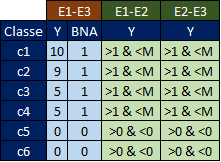
\includegraphics[scale=0.8]{img/tab_trechos_maiores.png}
		\caption{Exemplo simples}
		% Fonte:~\cite{khaksar2013genetic}}
		\label{fig: exemplo_sip}
	\end{center}
\end{figure}

Para o trecho $"E1-E3"$, note que quando $Y \neq 0$, $BNA = 1$ e quando $Y = 0$, $BNA = 0$ (controlado pela restrição \ref{eq: m1_activ_bin_autho}). Agora observe que, quando$ BNA = 1$ para uma certa classe, os trechos $E1-E2$ e $E2-E3$ assumem valores entre 1 e um número suficientemente grande ($1 \le Y \leq M$), o que indica que os assentos a serem disponibilizados para essa classe nesses trechos não podem ser zero. Por outro lado, quando $BNA = 0$, os trechos menores devem zerar a classe correspondente com ($0 \leq Y \leq 0$), ou seja, não se deve disponibilizar assentos com essa classe (controlado pela restrição \ref{eq: m1_autho_igualar_trecho_maior}). Deve-se esclarecer que os trechos menores apenas imitam o comportamento da classe maior e não os valores que esta assume.

As restrições de \ref{eq: m1_ini_assig} e \ref{eq: m1_ini_disponi} são usadas para inicializar a restrição \ref{eq: m1_disponi} quando \(i = 1\). E as restrições de \ref{eq: m1_dom_assig} a \ref{eq: m1_dom_bin_nadja} representam o domínio das variáveis.

\section{Segunda modelagem matemática}\label{sec:modelo2}

Vamos considerar novamente uma versão simplificada do problema. Na verdade, para esta modelagem, serão levadas em conta as mesmas variáveis do primeiro modelo, exceto a variável de disponibilidade \(A\), conforme mostrado a seguir:

\noindent $x_{ij}$: Quantidade de assentos que será disponibilizada para venda no trecho com origem em $i$ e destino em $j$, onde $j>i$ \\
\noindent $P_{ij}$: Preço da passagem no trajeto com origem em $i$ e destino em $j$ \\
\noindent $Q$: Capacidade do trem

\noindent Assim, a função objetivo e as restrições são como segue:

$FO: max \quad x_{12}P_{12} + x_{13}P_{13} + x_{14}P_{14} + x_{23}P_{23} + x_{24}P_{24} + x_{34}P_{34}$

s.a.

\noindent{\it Restrições para estações de origem}

Estação 1: $x_{12} + x_{13} + x_{14} \leq Q $ \\
\indent Estação 2: $x_{23} + x_{24}  \leq  Q $ \\
\indent Estação 3: $x_{34} \leq Q $

\noindent{\it Restrições para estações de destino}

Estação 2: $x_{12} \leq Q $ \\
\indent Estação 3: $x_{13} + x_{23}  \leq  Q $ \\
\indent Estação 4: $x_{14} + x_{24} + x_{34} \leq Q $

Observe que esta formulação é baseada nos modelos de transporte, onde as estações de origem seriam os depósitos e estão restritas por sua capacidade (capacidade do trem), e as estações de destino seriam os destinos e estão restritas, neste caso, pela mesma capacidade do trem e não pela demanda de cada destino.

Esta formulação garante que sempre será disponibilizada, no máximo, a capacidade do trem tanto para cada saída quanto para cada chegada do trem. Imagine uma solução viável como a mostrada na figura \ref{fig: fig2}.

\begin{figure}[h]
	\begin{center}
		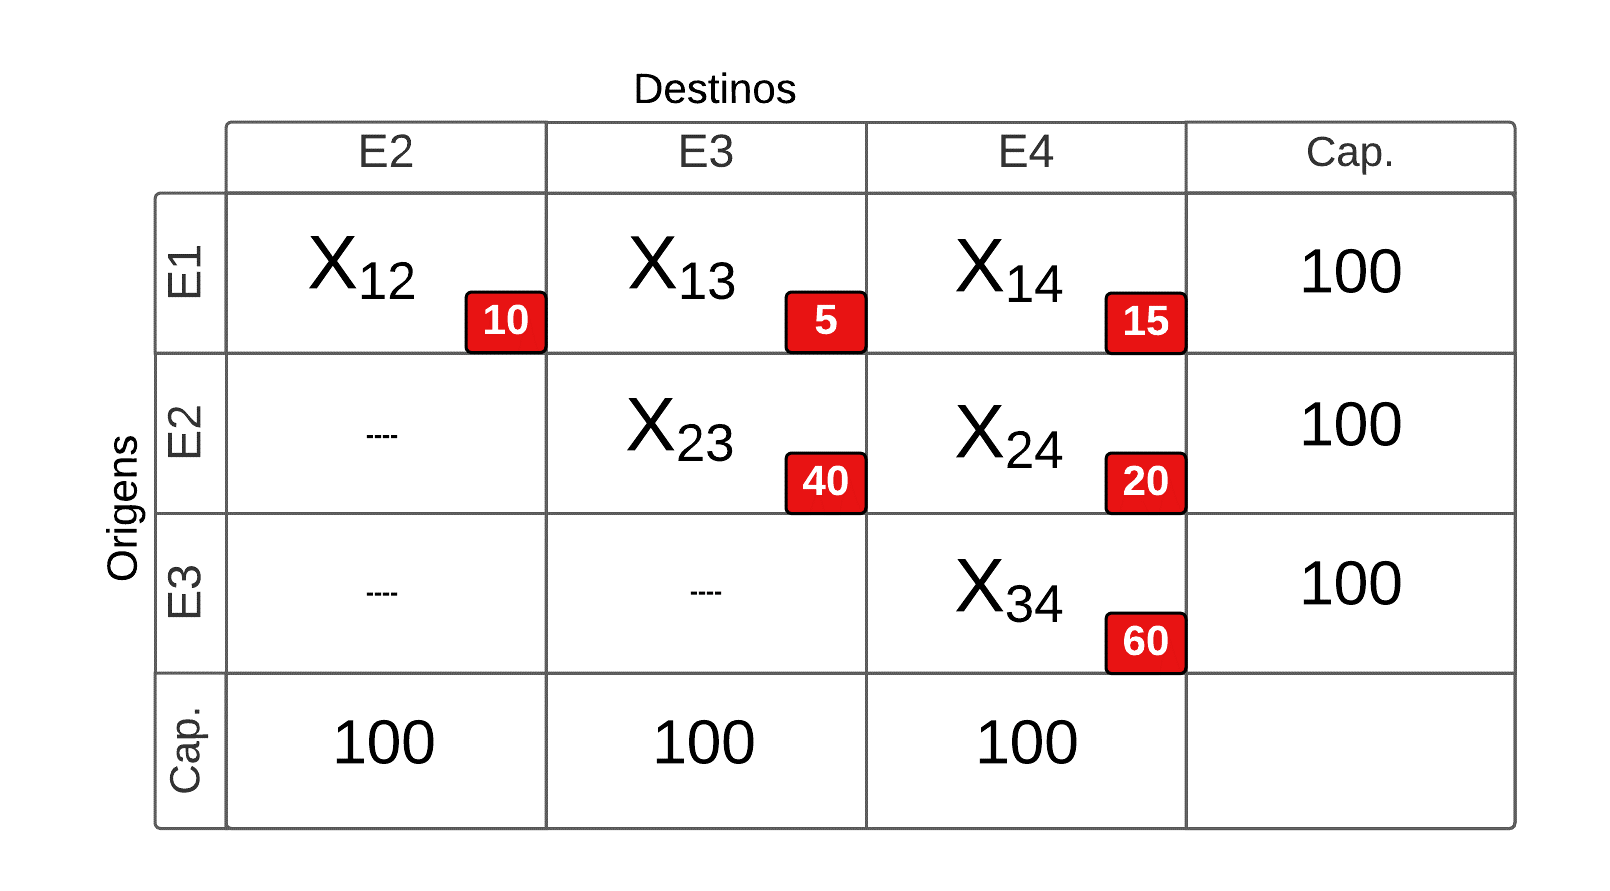
\includegraphics[scale=0.4]{img/fig3.png}
		\caption{Solução factível para o problema simplificado}
		% Fonte:~\cite{khaksar2013genetic}}
		\label{fig: fig3}
	\end{center}
\end{figure}

Observe que os valores das variáveis são os mesmos que foram mostrados na figura \ref{fig: fig3}. E ainda todas as restrições, tanto por linha quanto por coluna (por origens e por destinos), continuam sendo atendidas.

\begin{table}[h]
	\centering
	\small
	\begin{tabular}{p{2cm} p{9.5cm} p{3.2cm}}
		\toprule
		\textbf{Definição} & \textbf{Notação}                                                                                                                                            & \textbf{Domínio}                             \\ \midrule
		\multicolumn{3}{l}{\textbf{Conjuntos}}                                                                                                                                                                                          \\ \midrule
		$OD$               & Conjunto de Trechos com itinerario                                                                                                                          &                                              \\
		$NAD$              & Conjunto de Trechos que NÃO são Adjacentes e que tem itinerario                                                                                             &                                              \\
		$BRI_{(o,d)}$      & Conjunto de Trechos contidos dentro de cada trecho $(o,d)$ NÃO Adjacente                                                                                    &                                              \\
		$V$                & Conjunto de Cabines do trem                                                                                                                                 &                                              \\
		$K_v$              & Conjunto de Classes de Control de cada cabine em $V$                                                                                                        &                                              \\
		$T$                & Conjunto de Check-Points (Períodos)                                                                                                                         &                                              \\ \midrule
		\multicolumn{3}{l}{\textbf{Parâmetros}}                                                                                                                                                                                         \\ \midrule
		$Q$                & Capacidade do trem                                                                                                                                          &                                              \\
		$P_{ijvk}$         & Preços  das passagem no Trecho $(i,j)$, Cabine $v$ e Classe de Control $k$                                                                                  & $(i,j) \in OD,v \in V, k \in K_v$            \\
		$D_{ijvkt}$        & Demanda  das passagem no Trecho $(i,j)$, Cabine $v$ e Classe de Control $k$                                                                                 & $(i,j) \in OD,v \in V, k \in K_v, t \in T$   \\ \midrule
		\multicolumn{3}{l}{\textbf{Variáveis de decisão}}                                                                                                                                                                               \\ \midrule
		$X_{ijvkt}$        & Quantidade de passagem atribuídos no trecho $(i,j)$, cabine $v$ e com classe de control $k$ no período $t$                                                  & $(i,j) \in OD, v \in V, k \in K_v, t \in T$  \\
		$Y_{ijvkt}$        & Quantidade de passagem autorizados no trecho $(i,j)$, cabine $v$ e com classe de control $k$ no período $t$                                                 & $(i,j) \in OD, v \in V, k \in K_v, t \in T$  \\
		$BNA_{ijvkt}$      & É uma variavel binaria que toma o valor de 1 quando $Y_{ijvkt} \neq 0$ e toma  valor de 0 caso contrario, aplica-se apenas a trechos que não são adjacentes & $(i,j) \in NAD, v \in V, k \in K_v, t \in T$ \\
		\bottomrule
	\end{tabular}
	\caption{Notação matemática}
	\label{tab: m2_definicao}
\end{table}
\begin{align}
	 & Max \quad Z = \sum_{(i,j)\in OD} \sum_{v\in V} \sum_{k\in K_v} \sum_{t\in T} P_{ijvk} X_{ijvkt}                                 \label{eq: m2_fo}                          \\
	 & \text{s.a.}  \notag                                                                                                                                                        \\
	 & \sum_{(i,j)\in OD}\sum_{v\in V}\sum_{k\in K_v}\sum_{t\in T}X_{ijvkt} \leq Q , \quad \forall j / j>1, i<j                        \label{eq: m2_cap_assig_destino}           \\
	 & \sum_{(i,j)\in OD}\sum_{v\in V}\sum_{k\in K_v}\sum_{t\in T}X_{ijvkt} \leq Q , \quad \forall i / i<n, j>i                        \label{eq: m2_cap_assig_origem}            \\
	 & Y_{ijvkt} \geq Y_{i,j,v,k+1,t},  \quad \forall (i,j),v,k,t / i < j, k < \lVert K_v \rVert,  P_{ijvk} \geq P_{i,j,v,k+1}         \label{eq: m2_jerar_class}                 \\
	 & X_{ijvkt} \leq D_{ijvkt},  \quad \forall (i,j),v,k,t/ i < j                                                                     \label{eq: m2_assig_menor_dem}             \\
	 & \sum_{(i,j) \in OD}\sum_{v\in V}\sum_{t\in T} Y_{i,j,v,k,t} \leq Q, \quad  k = min\{K_v\}, \forall i \in OD                     \label{eq: m2_cap_autho_1er_class}         \\
	 & Y_{i,j,v,k,t} \geq  X_{i,j,v,k,t},  \quad k = max\{K_v\}, \forall(i,j),v,t                                                      \label{eq: m2_autho_mayor_assig_1er_class} \\
	 & Y_{i,j,v,k,t} \geq  X_{i,j,v,k,t} + Y_{i,j,v,k + 1,t} , \forall(i,j),v, k, t / k < \lVert K_v\rVert                             \label{eq: m2_autho_mayor_assig_mas_autho} \\
	 & BNA_{o,d,v,k,t} \leq Y_{o,d,v,k,t} \leq BNA_{o,d,v,k,t} Q, \quad  \forall (o,d)\in NAD, v, k, t                                 \label{eq: m2_activ_bin_autho}             \\
	 & BNA_{o,d,v,k,t} \leq Y_{i,j,v,k,t} \leq BNA_{o,d,v,k,t} Q, \quad  \forall (o,d)\in NAD, (i,j) \in BRI_{(o,d)}, v,k,t            \label{eq: m2_autho_igualar_trecho_maior}  \\
	 & X_{ijvkt} \in \mathbb{Z}^+                                                                                                      \label{eq: m2_dom_assig}                  %\\
\end{align}
\begin{align}
	& Y_{ijvkt} \in \mathbb{Z}^+                                                                                                      \label{eq: m2_dom_autho}                   \\
	& BNA_{ijvkt} \in \{0,1\}                                                                                                         \label{eq: m2_dom_bin_nadja}
\end{align}

Como já foi mencionado, nesta formulação modificamos as restrições que controlam as variáveis asseguradas X, ou seja, mudamos as restrições 1 e 2 do primeiro modelo e eliminamos a variável de decisão Ai.

% \end{adjustwidth}
%Note que, na definição, não temos mais a variável de decisão de disponibilidade \(A_i\). Neste caso, a equação \ref{eq: m2_fo} representa a função objetivo que esta tentando maximizar a soma do produto entre as quantidades seguradas e os preços das mesmas, ou seja, estamos maximizando a receita em função das quantidades dos assentos que estão assegurados.

%A restrição \ref{eq: m2_cap_assig_destino} garante que a quantidade total de assentos autorizados para cada destino seja a quantidade máxima de assentos do trem para todas as classes e todos os períodos.
%A restrição \ref{eq: m2_cap_assig_origem} garante que a quantidade de assentos autorizados para cada origem seja no máximo a capacidade do trem para todas as classes e todos os períodos.
%As restrições de \ref{eq: m2_cap_autho_1er_class} a \ref{eq: m2_dom_autho} representam o mesmo que o primeiro modelo já exposto.\\

Para este caso, as restrições \ref{eq: m2_cap_assig_destino} e \ref{eq: m2_cap_assig_origem} representam a generalização do problema simplificado, onde a primeira garante que a quantidade de assentos autorizados para venda não viole a capacidade do trem ao chegar a cada estação de destino; e a segunda garante que a quantidade de assentos autorizados respeite a capacidade do trem no momento de sair de cada estação de origem. O restante das restrições foi explicado na formulação 1.